\documentclass{article}

\usepackage{tikz}
\usepackage{pgfplots}
\begin{document}

\begin{figure}
\centering
 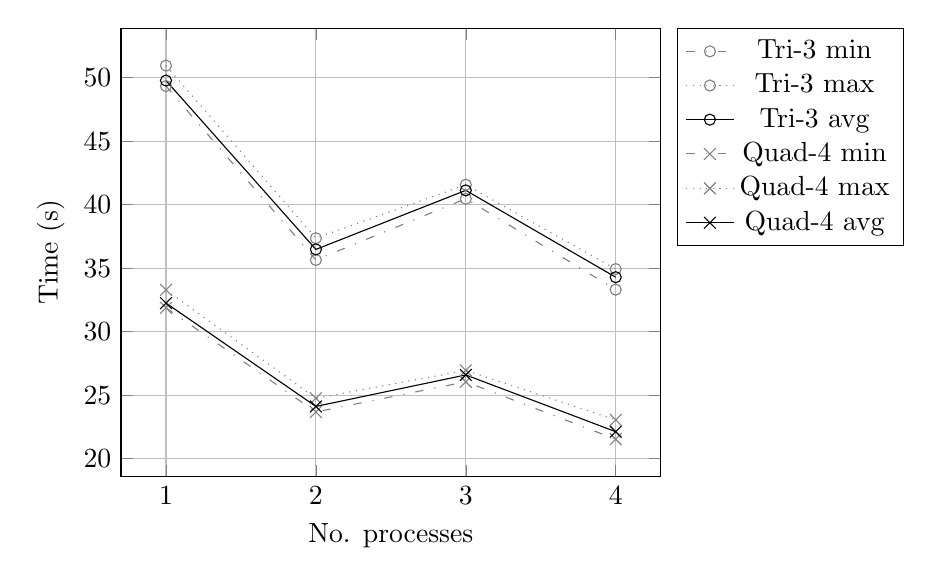
\begin{tikzpicture}
  \begin{axis}[xlabel=No. processes,
			   ylabel=Time (s),
			   xtick={1,2,3,4},
			   ytick={50,45,40,35,30,25,20},
			   grid=major,
			   legend pos=outer north east]
	\addplot[mark=o,loosely dashdotted,gray,mark options={solid}] plot coordinates {
		(1,49.35)
		(2,35.65)
		(3,40.47)
		(4,33.31)
	};  
	\addlegendentry{Tri-3 min}
	\addplot[mark=o,dotted,gray,mark options={solid}] plot coordinates {
		(1,50.96)
		(2,37.36)
		(3,41.57)
		(4,34.93)
	};  
	\addlegendentry{Tri-3 max}
	\addplot[mark=o,black] plot coordinates {
		(1,49.78)
		(2,36.48)
		(3,41.13)
		(4,34.29)
	};  
	\addlegendentry{Tri-3 avg}
%%%%%%%%%%%%%%%%%%%%%%%%%%%%%%%%%%%%%%%%%%%%%%%%%%%%%%%%%	
	\addplot[mark=x,loosely dashdotted,gray,mark options={scale=1.5,solid}] plot coordinates {
		(1,31.88)
		(2,23.67)
		(3,26.05)
		(4,21.53)
	};
	\addlegendentry{Quad-4 min}
	\addplot[mark=x,dotted,gray,mark options={scale=1.5,solid}] plot coordinates {
		(1,33.29)
		(2,24.75)
		(3,26.95)
		(4,23.05)
	};
	\addlegendentry{Quad-4 max}
	\addplot[mark=x,black,mark options={scale=1.5}] plot coordinates {
		(1,32.25)
		(2,24.11)
		(3,26.59)
		(4,22.12)
	};
	\addlegendentry{Quad-4 avg}
	\end{axis}
	\end{tikzpicture}
	\caption{Solver Times}
	\label{fig:solver-times}
\end{figure}

\begin{figure}
	\centering
	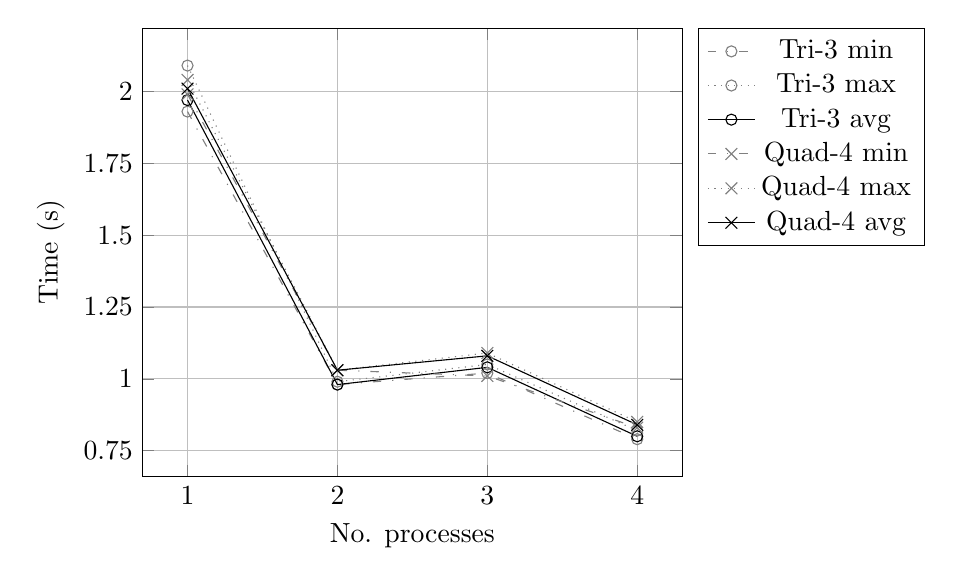
\begin{tikzpicture}
	\begin{axis}[xlabel=No. processes,
	ylabel=Time (s),
	xtick={1,2,3,4},
	ytick={2,1.75,1.5,1.25,1,0.75},
	grid=major,
	legend pos=outer north east]
	\addplot[mark=o,loosely dashdotted,gray,mark options={solid}] plot coordinates {
		(1,1.93)
		(2,0.98)
		(3,1.02)
		(4,0.79)
	};  
	\addlegendentry{Tri-3 min}
	\addplot[mark=o,dotted,gray,mark options={solid}] plot coordinates {
		(1,2.09)
		(2,0.99)
		(3,1.05)
		(4,0.82)
	};  
	\addlegendentry{Tri-3 max}
	\addplot[mark=o,black] plot coordinates {
		(1,1.97)
		(2,0.98)
		(3,1.04)
		(4,0.8)
	};  
	\addlegendentry{Tri-3 avg}
	%%%%%%%%%%%%%%%%%%%%%%%%%%%%%%%%%%%%%%%%%%%%%%%%%%%%%%%%%	
	\addplot[mark=x,loosely dashdotted,gray,mark options={scale=1.5,solid}] plot coordinates {
		(1,1.99)
		(2,1.03)
		(3,1.01)
		(4,0.83)
	};
	\addlegendentry{Quad-4 min}
	\addplot[mark=x,dotted,gray,mark options={scale=1.5,solid}] plot coordinates {
		(1,2.04)
		(2,1.03)
		(3,1.09)
		(4,0.85)
	};
	\addlegendentry{Quad-4 max}
	\addplot[mark=x,black,mark options={scale=1.5}] plot coordinates {
		(1,2.01)
		(2,1.03)
		(3,1.08)
		(4,0.84)
	};
	\addlegendentry{Quad-4 avg}
	\end{axis}
	\end{tikzpicture}
	\caption{Solver Times}
	\label{fig:assembly-times}
\end{figure}

\begin{figure}
	\centering
	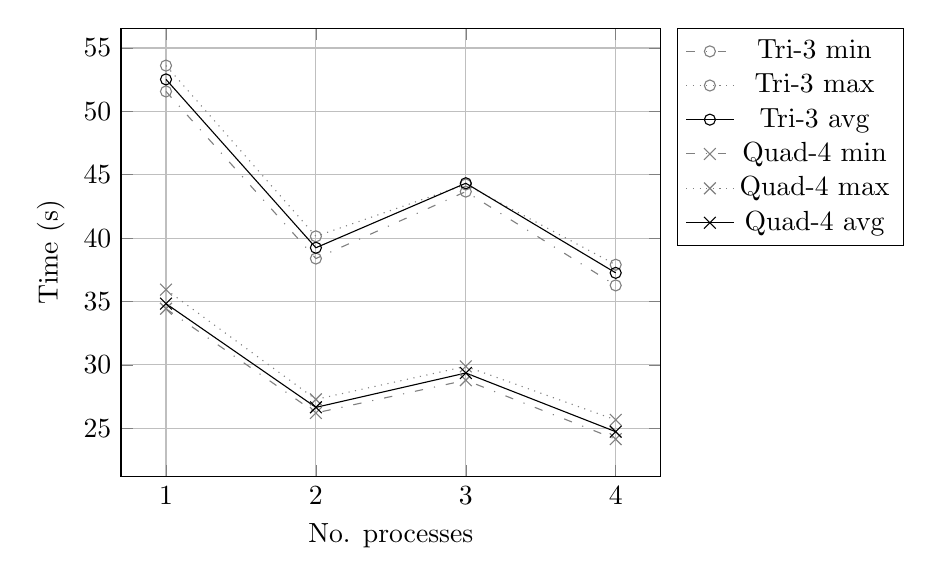
\begin{tikzpicture}
	\begin{axis}[xlabel=No. processes,
	ylabel=Time (s),
	xtick={1,2,3,4},
	ytick={55,50,45,40,35,30,25},
	grid=major,
	legend pos=outer north east]
	\addplot[mark=o,loosely dashdotted,gray,mark options={solid}] plot coordinates {
		(1,51.57)
		(2,38.39)
		(3,43.67)
		(4,36.27)
	};  
	\addlegendentry{Tri-3 min}
	\addplot[mark=o,dotted,gray,mark options={solid}] plot coordinates {
		(1,53.61)
		(2,40.14)
		(3,44.23)
		(4,37.90)
	};  
	\addlegendentry{Tri-3 max}
	\addplot[mark=o,black] plot coordinates {
		(1,52.52)
		(2,39.24)
		(3,44.33)
		(4,37.26)
	};  
	\addlegendentry{Tri-3 avg}
	%%%%%%%%%%%%%%%%%%%%%%%%%%%%%%%%%%%%%%%%%%%%%%%%%%%%%%%%%	
	\addplot[mark=x,loosely dashdotted,gray,mark options={scale=1.5,solid}] plot coordinates {
		(1,34.43)
		(2,26.21)
		(3,28.79)
		(4,24.14)
	};
	\addlegendentry{Quad-4 min}
	\addplot[mark=x,dotted,gray,mark options={scale=1.5,solid}] plot coordinates {
		(1,35.94)
		(2,27.28)
		(3,29.88)
		(4,25.66)
	};
	\addlegendentry{Quad-4 max}
	\addplot[mark=x,black,mark options={scale=1.5}] plot coordinates {
		(1,34.83)
		(2,26.65)
		(3,29.36)
		(4,24.73)
	};
	\addlegendentry{Quad-4 avg}
	\end{axis}
	\end{tikzpicture}
	\caption{Solver Times}
	\label{fig:overall-times}
\end{figure}

\end{document}